\utilchap{smokezip - A utility for reducing FDS file sizes}
\label{ch:smokezip}

\begin{figure}[bph]
\centerline{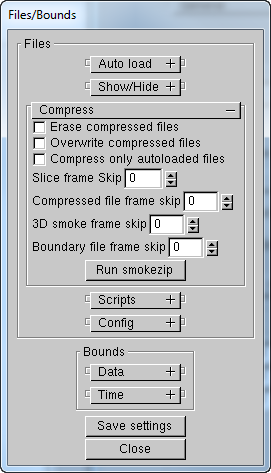
\includegraphics[width=1.881944in]{\SMVUGfigdir/figBOUNDcompress}\ }
\caption[Compress Files and Autoload dialog box.] {File/Bounds dialog
box showing compression and autoload options.  3D smoke,  boundary and slice
files may be compressed using Smokezip.  All currently loaded
files may be loaded automatically when Smokeview first starts by
selecting the autoload checkbox.}\ \label{figBOUNDScompress}
\end{figure}

3D smoke, boundary, isosurface and slice files may be compressed
using the utility Smokezip.  FDS data files may also be compressed
from within Smokeview using the compression menu item found in the
{\em Load/Unload}\ menu.  File compression may also be activated
from the Compressions, Autoload section of the File/Bounds
dialog box illustrated in Fig. \ref{figBOUNDScompress}.
Compression is performed using the ZLIB compression library (see
\hhref{http://www.zlib.org}). Smokeview compresses files in the
background allowing one to continue visualizing cases.  Smokeview
adds the label {\em ZLIB}\ to Load menu entries for any file that
has been compressed. Smokezip adds the extension .svz to any FDS
data file that has been compressed.

The usage for Smokezip (which may be obtained by typing Smokezip~-help at a command line) is

\lstinputlisting{SCRIPT_FIGURES/smokezip.help}

Smokezip either determines data bounds itself (if the -bounds option was specified)
or uses min and max values found in the casename.ini
file.  These bounds are used to map four byte floating point data
found in FDS data files to one byte color indices used by
Smokeview.  The algorithms for determining
the data mappings used by Smokeview and Smokezip are identical so it
should result in the same views.

Particle files may be converted to isosurface files using the {\tt
-part2iso}\ option as in {\tt Smokezip -part2iso casename}.  The
resulting isosurface file highlights particle boundaries (where
particle density is 0.5 particles per grid cell). These isosurface
files are accessible in the .smv file named {\tt
casename\_smvzip.smv}.
